% !TeX program = xelatex
\documentclass[10pt]{beamer}

\usetheme{metropolis}

\usepackage{pgfplots}
\usepgfplotslibrary{fillbetween}
\usepackage{pgfopts}
\usepackage{amsmath}
\usepackage{structuralanalysis}
\usepackage{tikz}
\usepackage{tikz-3dplot}
\usepackage{chngcntr}
\usepackage{wasysym}
\usepackage{mathtools}
\usepackage{alphalph}
\usepackage{xcolor}
\usepackage[showdow=false, en-US]{datetime2}
\usepackage{hyperref}

\newcommand{\highlight}[1]{%
	\colorbox{red!50}{$\displaystyle#1$}}

\setcounter{lecture}{15}
\counterwithin{equation}{lecture}
\makeatletter
\def\user@resume{resume}
\def\user@intermezzo{intermezzo}
%
\newcounter{previousequation}
\newcounter{lastsubequation}
\newcounter{savedparentequation}
\setcounter{savedparentequation}{1}
% 
\renewenvironment{subequations}[1][]{%
	\def\user@decides{#1}%
	\setcounter{previousequation}{\value{equation}}%
	\ifx\user@decides\user@resume 
	\setcounter{equation}{\value{savedparentequation}}%
	\else  
	\ifx\user@decides\user@intermezzo
	\refstepcounter{equation}%
	\else
	\setcounter{lastsubequation}{0}%
	\refstepcounter{equation}%
	\fi\fi
	\protected@edef\theHparentequation{%
		\@ifundefined {theHequation}\theequation \theHequation}%
	\protected@edef\theparentequation{\theequation}%
	\setcounter{parentequation}{\value{equation}}%
	\ifx\user@decides\user@resume 
	\setcounter{equation}{\value{lastsubequation}}%
	\else
	\setcounter{equation}{0}%
	\fi
	\def\theequation  {\theparentequation  \alph{equation}}%
	\def\theHequation {\theHparentequation \alph{equation}}%
	\ignorespaces
}{%
%  \arabic{equation};\arabic{savedparentequation};\arabic{lastsubequation}
\ifx\user@decides\user@resume
\setcounter{lastsubequation}{\value{equation}}%
\setcounter{equation}{\value{previousequation}}%
\else
\ifx\user@decides\user@intermezzo
\setcounter{equation}{\value{parentequation}}%
\else
\setcounter{lastsubequation}{\value{equation}}%
\setcounter{savedparentequation}{\value{parentequation}}%
\setcounter{equation}{\value{parentequation}}%
\fi\fi
%  \arabic{equation};\arabic{savedparentequation};\arabic{lastsubequation}
\ignorespacesafterend
}
\makeatother
\title{AE 737 - Mechanics of Damage Tolerance}
\subtitle{Lecture \arabic{lecture}}
\date{Last Updated: \today\ at \DTMcurrenttime}
\author{Dr. Nicholas Smith}
\institute{Wichita State University, Department of Aerospace Engineering}
% \titlegraphic{\hfill\includegraphics[height=1.5cm]{logo/logo}}

\begin{document}

\maketitle
\begin{frame}{schedule}
	\begin{itemize}
		\item 22 Mar - Stress based fatigue, Homework 6 assigned
		\item 24 Mar - Stress based fatigue
		\item 29 Mar - Influence of notches on fatigue, Homework 7 assigned, Homework 6 due
		\item 31 Mar - Strain based fatigue, project abstract due
	\end{itemize}
\end{frame}

\begin{frame}
  \frametitle{outline}
  \setbeamertemplate{section in toc}[sections numbered]
  \tableofcontents[hideallsubsections]
\end{frame}

\section{fatigue}

\begin{frame}{fatigue}
	\begin{itemize}
		\item We refer to damage from repeated, or cyclic loads as fatigue damage
		\item Some of the earliest work on fatigue began in the 1800's
		\item Chains, railway axles, etc.
		\item An estimated 80\% of failure expenses are due to fatigue
	\end{itemize}
\end{frame}

\begin{frame}{fatigue}
	\begin{itemize}[<+->]
		\item There are three main approaches to fatigue analysis
		\item Stress based fatigue analysis
		\item Strain based fatigue analysis
		\item Fracture mechanics fatigue analysis
	\end{itemize}
\end{frame}

\begin{frame}{stress based fatigue}
	\begin{itemize}[<+->]
		\item One of the simplest assumptions we can make is that a load cycles between a constant maximum and minimum stress value
		\item This is a good approximation for many cases (axles, for example) and can also be easily replicated experimentally
		\item This is referred to as constant amplitude stressing
	\end{itemize}
\end{frame}

\begin{frame}{constant amplitude stressing}
	\begin{figure}
		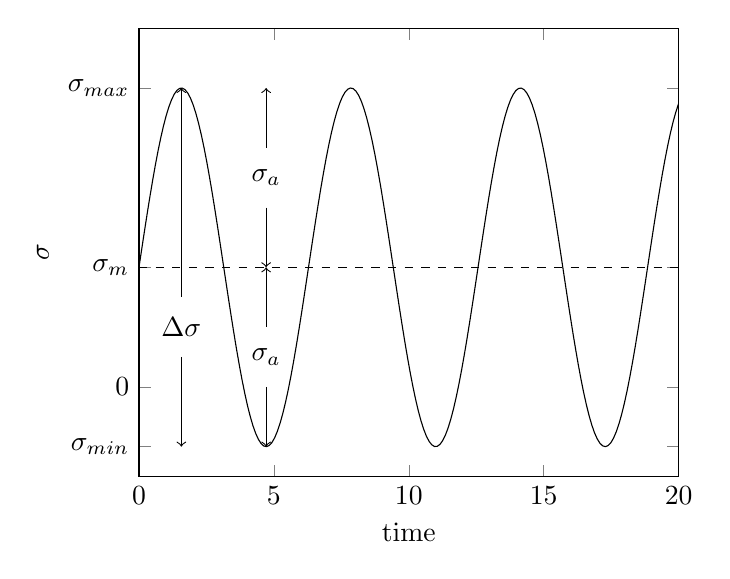
\begin{tikzpicture}
		\begin{axis}[
		domain=0:20,
		samples=200,
		xmin=0,   xmax=20,
		ymin=-3,   ymax=12,
		ylabel=$\sigma$,
		xlabel=time,
		ytick={-2, 0, 4, 10},
		yticklabels={$\sigma_{min}$, 0, $\sigma_m$, $\sigma_{max}$}]
		\addplot [color=black,mark=none] {6*sin(deg(x)) + 4};
		\addplot [color=black,style=dashed,mark=none] coordinates { (0,4) (20,4)};
		\draw[<-] (axis cs: 3.14159/2,10) -- (axis cs: 3.14159/2,3);
		\draw[->] (axis cs: 3.14159/2,1) -- (axis cs: 3.14159/2,-2);
		\draw node at (axis cs: 3.14159/2,2) {$\Delta \sigma$};
		\draw[<-] (axis cs: 3*3.14159/2,4) -- (axis cs: 3*3.14159/2,2);
		\draw[->] (axis cs: 3*3.14159/2,0) -- (axis cs: 3*3.14159/2,-2);
		\draw node at (axis cs: 3*3.14159/2,1) {$\sigma_a$};
		\draw[<-] (axis cs: 3*3.14159/2,10) -- (axis cs: 3*3.14159/2,8);
		\draw[->] (axis cs: 3*3.14159/2,6) -- (axis cs: 3*3.14159/2,4);
		\draw node at (axis cs: 3*3.14159/2,7) {$\sigma_a$};
		\end{axis}
		\end{tikzpicture}
	\end{figure}
\end{frame}

\begin{frame}{constant amplitude stressing}
	\begin{itemize}[<+->]
		\item $\Delta \sigma$ is known as the stress range, and is the difference between max and min stress
		\item $\sigma_m$ is the mean stress, and can sometimes be zero, but this is not always the case
		\item 
	\end{itemize}
\end{frame}
\end{document}
